\chapter{Tor wizyjny}
\label{cha:torwizyjny}

Kolejnym krokiem realizacji projektu była implementacja podstawowych zadań przetwarzania obrazu w logice rekonfigurowalnej układu heterogenicznego. Rozpoczęto od stworzenia podstawowego toru wizyjnego pobierającego obraz z wejścia HDMI i wysyłającego bez zmian na wyjście VGA. Następnie stworzono moduły pozwalające na realizację algorytmu śledzenia przez detekcję.

\section{Podstawowe przesyłanie obrazu}
\label{sec:podstawoweprzesylanieobrazu}
Tor wizyjny nie wykonujący żadnych zmian w obrazie pozwoli nam na określenie czy dane są poprawnie odbierane z kamery i poprawnie wysyłane do monitora. Stanowić on będzie również bazę dla dowolnego innego realizowanego algorytmu przetwarzania obrazu. Konieczna jest więc pewność, że działa poprawnie. Musi on realizować następujące zadania:
\begin{enumerate}
\item Odbieranie danych ze złącza DVI.
\item Konwersja danych odebranych ze złącza DVI do przestrzeni barw RGB i sygnałów synchronizacyjnych.
\item Konwersja przestrzeni barw RGB i sygnałów synchronizacyjnych do VGA.
\item Wysłanie danych do złącza VGA.
\end{enumerate}
Zadania te są realizowane przez moduły dostarczane przez firmę \textit{Digilent}, producenta platformy obliczeniowej. Moduły połączone zostały za pomocą diagramu w programie \textit{Vivado}. Diagram, w porównaniu do pliku języka Verilog, zwiększa przejrzystość połączeń między modułami oraz zmniejsza ryzyko błędu np. w nazwie portu.

\begin{figure}[h]
	\centering
	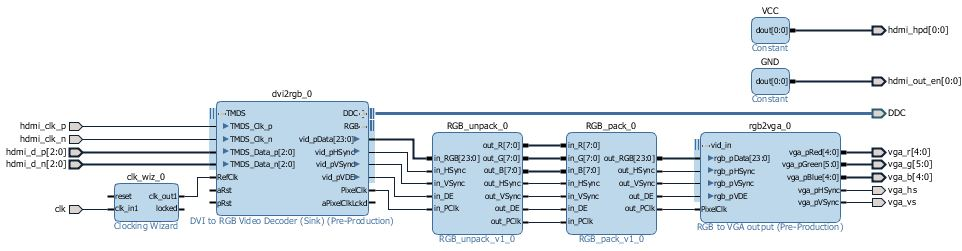
\includegraphics[width=4in]{Tor_wizyjny.jpg}
	\captionsource{Podstawowy tor wizyjny.}{Własne}
\end{figure}

\paragraph*{}
Testy rozpoczęto od podłączenie wyjścia HDMI laptopa do wejścia HDMI płytki ZYBO oraz podłączenia monitora do wyjścia VGA ZYBO. W tak połączonym układzie obraz był wyświetlany poprawnie. Następnie źródło obrazu zamieniono na docelową kamerę. Tym razem żadem obraz nie został wyświetlony na ekranie monitora. W celu znalezienia i naprawy problemu postanowiono w torze wizyjnym włączyć opcję \textit{debug} dla części węzłów. Dzięki temu można podglądać sygnały już w działającym układzie. Ustalono, że problem jest z modułem odbierającym dane z wejścia HDMI - \textit{dvi2rgb}. Problem udało się naprawić aktualizując go z wersji 1.2 do wersji 1.6 oraz zmieniając ustawienia zegara taktującego oraz domyślnej rozdzielczości przetwarzanego obrazu.

\section{Śledzenie przez detekcję}
\label{sec:sledzenieprzezdetekcje}

Śledzenie przez detekcję zostało zrealizowane na podstawie koloru śledzonego obiektu. Jako parametr modułu detekcji podawany jest zakres kolorów w przestrzeni barw RGB, które mają być traktowane jako należące do obiektu. Pikselowi, którego kolor mieści się w podanym zakresie przypisywana jest wartość 1, a pozostałym 0. Pod nadaniu wartości wszystkim pikselom kadru obliczany jest środek ciężkości obrazu. Wyznaczony środek ciężkości jest środkiem śledzonego obiektu. Punkt ten zaznaczany jest na obrazie wyjściowym za pomocą dwóch czerwonych linii - poziomej i pionowej. Podczas testów wykrywany był następujący zakres przestrzeni barw RGB, odpowiadający kolorowi zielonemu:
\begin{equation}
R \in [0,30]
\end{equation}
\begin{equation}
G \in [40,255]
\end{equation}
\begin{equation}
B \in [0,30]
\end{equation}

\begin{figure}[h]
	\centering
	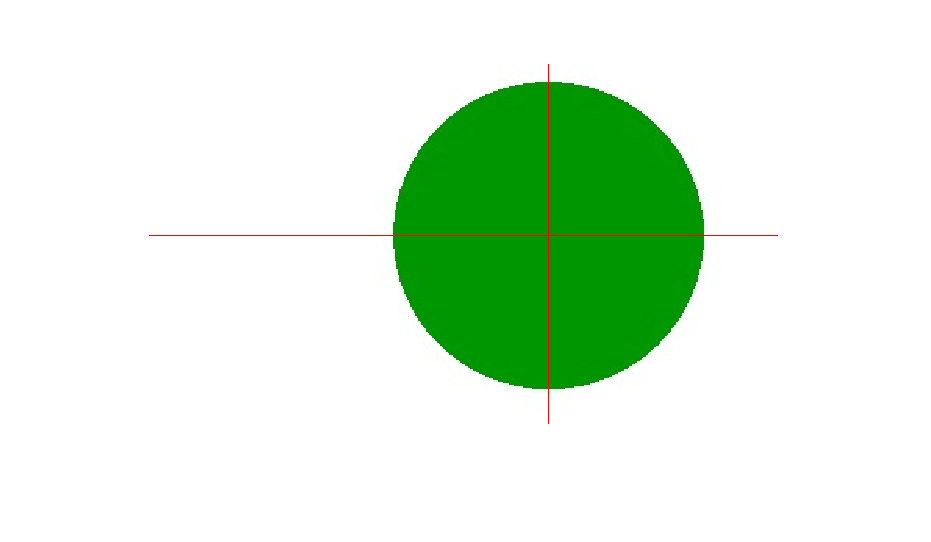
\includegraphics[width=4in]{kolo_srodek.eps}
	\captionsource{Przykładowy wynik działania algorytmu.}{Własne}
\end{figure}

Testy były wykonywane zarówno dla obrazu z komputera PC jak i kamery. Należy zwrócić uwagę na niską efektywność tej metody dla obrazu z kamery. Spowodowane jest to szumami oraz bardzo dużą zależnością rozpoznanego koloru od natężenia i rodzaju światła.

\section{Komunikacja PL-PS}
\label{komunikacjapl-ps}

Połączono wykonany w tym rozdziale tor wizyjny z wyznaczaniem środka ciężkości z komunikacją zaimplementowaną w rozdziale \ref{cha:komunikacja}. Komunikacja pomiędzy procesorem ARM a FPGA odbywa się z użyciem modułu \textit{AXI Lite}. Do procesora wysyłane są współrzędne wyznaczonego środka ciężkości śledzonego obiektu. Kiedy dane są gotowe do odczytu, sygnał oznaczający wysłanie danych do procesora zmienia wartość logiczna z \(0\) na \(1\). Od narastającego zbocza tego sygnału zgłaszane jest przerwanie, w którym aktualizowana jest zmienna odpowiedzialna za położenie celu, czyli wartości zadane serwomechanizmów. W procesorze odebrane współrzędne przeliczone zostają na uchyby regulacji kątów na podstawie rozdzielczości obrazu i kątów nagrywania kamery. Założono, że odległość pikseli od środka obrazu jest proporcjonalna do kąta. Założenie to nie jest słuszne, lecz pozwala pominąć znaczną ilość testów, które należałoby przeprowadzić, aby wyznaczyć tą funkcję. Obliczanie skomplikowanych funkcji matematycznych wymagałoby również znacznie więcej czasu procesora.